\documentclass{article}
\usepackage{algorithm}
\usepackage{algpseudocode}
\usepackage{amsmath,amssymb,amsthm}
\usepackage{graphicx}
\usepackage[margin=1in]{geometry}
\usepackage{fancyhdr}
\usepackage{longtable}
\usepackage{lipsum}
\setlength{\parindent}{0pt}
\setlength{\parskip}{5pt plus 1pt}
\setlength{\headheight}{13.6pt}
\newcommand\question[2]{\vspace{.25in}\hrule\textbf{#1: #2}\hrule\vspace{.10in}}
\renewcommand\part[1]{\vspace{.10in}\textbf{(#1)}}
\newcommand\algo{\vspace{.10in}\textbf{Algorithm: }}
\newcommand\correctness{\vspace{.10in}\textbf{Correctness: }}
\newcommand\runtime{\vspace{.10in}\textbf{Running time: }}
\newcommand\pseudoCode{\vspace{.10in}\textbf{PseudoCode: }}
\newcommand*{\perm}[2]{{}^{#1}\!P_{#2}}
\newcommand*{\comb}[2]{{}^{#1}\!C_{#2}}
%\pagestyle{fancyplain}
%\lhead{\textbf{\NAME\ (\UID)}}
%\chead{\textbf{Hw\HWNUM}}
%\rhead{CS 6150, \today}
\title{CS6150 - Homework/Assignment-3}
\author{Arnab Das(u1014840)}
\usepackage[utf8]{inputenc}
\begin{document}
  \pagenumbering{gobble}
  \maketitle
  \newpage
  \pagenumbering{arabic}
  \newcommand\NAME{ARNAB DAS}
  \newcommand\UID{uxxxxxxx}
  \newcommand\HWNUM{3}

  \question{1}{easy relatives of 3-SAT}
	\part{a} Given a caluse of a 2-CNF formula $x_{1} \vee x_{2}$. Goal is to prove that this clause is logically equivalent to the clause $\bar{x_{1}} \Rightarrow x_{2}$.  The implication clause $\bar{x_{1}} \Rightarrow x_{2}$ means, if $\bar{x_{1}}$ is true, it implies $x_{2}$, else if $\bar{x_{1}}$ is false then the implication doesn't fires and the result is true. Thus, when $\bar{x_{1}}$ is false(or $x_{1}$ is true), the clause is always true regardless of $x_{2}$. When $\bar{x_{1}}$ is true, it implies the clause is determined by the result of $x_{2}$, that is if $x_{2}$ is true, then the result is true, and if $x_{2}$ is false, the result is false. Thus, if we make the truth table of $\bar{x_{1}} \Rightarrow x_{2}$, the table will look as below: \newline
\begin{table}[ht]
  \caption{Truth Table of $\bar{x_{1}} \Rightarrow x_{2}$}
  \centering
  \begin{tabular}{c c c }
  \hline\hline
  $\bar{x_{1}}$ & $x_{2}$ & $\bar{x_{1}} \Rightarrow x_{2}$ \\[0.5ex]
  \hline
  0 & 0 & 1 \\
  0 & 1 & 1 \\
  1 & 0 & 0 \\
  1 & 1 & 1 \\ [0.5ex]
  \end{tabular}
  \label{table:nonlin}
  \end{table}	  

Below is the truth table of $x_{1} \vee x_{2}$ \newline
\begin{table}[ht]
  \caption{Truth Table of $x_{1} \vee x_{2}$}
  \centering
  \begin{tabular}{c c c }
  \hline\hline
  $\bar{x_{1}}$ & $x_{2}$ & ${x_{1}} \vee x_{2}$ \\[0.5ex]
  \hline
  0 & 0 & 1 \\
  0 & 1 & 1 \\
  1 & 0 & 0 \\
  1 & 1 & 1 \\ [0.5ex]
  \end{tabular}
  \label{table:nonlin}
  \end{table}	 

  The truth tables of table-1 and table-2 are exactly the same thus implying that the clause $x_{1} \vee x_{2}$ is equivalent to $\bar{x_{1}} \Rightarrow x_{2}$. \newline

  \part{b} Suppose we have a 2-CNF formula, comprising of m-clauses. It is unsatisfiable if their exists a clause $(x_{i} \vee x_{j})$, such that we have combination like \newline
\begin{equation}
   (x_{i} \vee x_{j})\wedge \bar{x_{i}} \wedge \bar{x_{j}}
\end{equation}
This is unsatisfiable because, $\bar{x_{i}}$ and $\bar{x_{j}}$  will require an assignment of $x_{i}=0$ and $x_{j} = 0$ for them to be true. However, this assignment will result in $(x_{i} \vee x_{j})$ to be false and hence unsatisfiable. This above combination of clauses can be further decomposed into the following pieces for ease of analysis. \newline
	\hspace*{0.5cm} (1). $\bar{x_{i}}$ in a 2-cnf form will be generated if there exists a path such that $(\bar{x_{i}} \vee \bar{x_{i}})$ equivalent to $(x_{i} \Rightarrow \bar{x_{i}})$ is present. \newline
      \hspace*{0.5cm} (2).  $\bar{x_{j}}$ in a 2-cnf form will be generated if there exists a path such that $(\bar{x_{j}} \vee \bar{x_{j}})$ equivalent to $(x_{j} \Rightarrow \bar{x_{j}})$ is present. \newline
	\hspace*{0.5cm} (3). Also, $(x_{i} \vee x_{j})$ can be written in either form of $(\bar{x_{i}} \Rightarrow x_{j})$ and $(\bar{x_{j}} \Rightarrow x_{i})$ \newline

If we consider a directed graph, where each literal is a node(thus for n variables there will be 2n literals) and the clause $(a \Rightarrow b)$ indicates an edge from node 'a' to node 'b', then the above 4 clauses will result in the following connectivity.\newline

  \begin{figure}[h!]
   \centering
  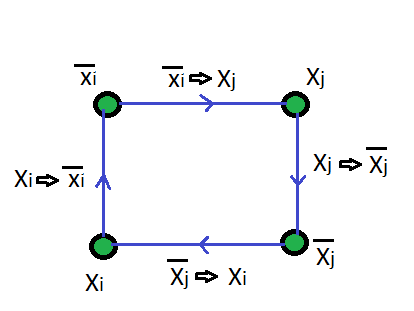
\includegraphics[width=5cm, height=5cm]{Prob1b}
  \caption{The cycle representation for unsatisfiability}
  \end{figure}

 As the figure suggests, the above formation of clauses results in a cycle. Note that the absence of any of the above caluses will result in a valid assignment, which from the perspective of the graph means that the cycle breaks resulting in a valid assignment. Existence of the cycle implies that there is a path from $x_{i}$ to $\bar{x_{i}}$ and from $\bar{x_{i}}$ to $x_{i}$, which essentially makes the 2-CNF formula unsatisfiable. (Proved)
Thus, satisfiability of a 2-CNF formula requires searching for the existence of such a cycle which can be easily found by using a Breath first search(BFS) which is of $O(|E|+|V|)$, where $|E| and |V|$ are the cardinality of the edges and vertices of the graph respectively. Thus, finding satisfiability of a 2-CNF formula is polynomial time.\newline

\part{c} A problem for 2-or-more  3SAT is defined as follows: Given a 3-CNF formula, $\phi$, an assignment is said to 2-or-more satisfy a clause iff atleast two of the literals in that clause are true for that assignment. \textbf {Goal:} To prove that there exists an assignment that 2-or-more 3SAT has a polynomial time algorithm. \newline

\textbf{Proof:} \newline
\textbf{Claim:} A 3-CNF clause, say, $(x_{i} \vee x_{j} \vee x_{k})$ , is 2-or-more satisfiable if the CNF breakdown of its $^3C_{2}$ combinations are satisfiable, that is, we can rewrite $(x_{i} \vee x_{j} \vee x_{k})$ as \newline
\begin{equation}
	(x_{i} \vee x_{j} \vee x_{k}) = (x_{i} \vee x_{j}) \wedge (x_{j} \vee x_{k}) \wedge (x_{k} \vee x_{i})
\end{equation}
This claim can be easily verified by constructing the truth tables of the lhs and the rhs of the equation as given below, \newline
\begin{table}[ht]
  \caption{Truth Table of 2-or-more($x_{i} \vee x_{j} \vee x_{k}$)}
  \centering
  \begin{tabular}{c c c c}
  \hline\hline
   $x_{i}$ & $x_{j}$ & $x_{k}$ & 2-or-more($x_{i} \vee x_{j} \vee x_{k}$) \\[0.5ex]
  \hline
  0 & 0 & 0 & 0 \\
  0 & 0 & 1 & 0 \\
  0 & 1 & 0 & 0 \\
  0 & 1 & 1 & 1 \\
  1 & 0 & 0 & 1 \\
  1 & 0 & 1 & 1 \\
  1 & 1 & 0 & 1 \\
  1 & 1 & 1 & 1 \\
  \end{tabular}
  \label{table:nonlin}
  \end{table}	  

\begin{table}[ht]
  \caption{Truth Table of $(x_{i} \vee x_{j}) \wedge (x_{j} \vee x_{k}) \wedge (x_{k} \vee x_{i})$}
  \centering
  \begin{tabular}{c c c c c c c}
  \hline\hline
  $x_{i}$ &  $x_{j}$ & $x_{k}$ & $(x_{i} \vee x_{j})$ & $(x_{j} \vee x_{k})$ & $(x_{k} \vee x_{i})$ & $(x_{i} \vee x_{j}) \wedge (x_{j} \vee x_{k}) \wedge (x_{k} \vee x_{i})$  \\[0.5ex]
  \hline
  0 & 0 & 0 & 0 & 0 & 0 & 0 \\
  0 & 0 & 1 & 0 & 1 & 1 & 0 \\
  0 & 1 & 0 & 1 & 1 & 0 & 0 \\
  0 & 1 & 1 & 1 & 1 & 1 & 1 \\
  1 & 0 & 0 & 1 & 1 & 1 & 1 \\
  1 & 0 & 1 & 1 & 1 & 1 & 1 \\
  1 & 1 & 0 & 1 & 1 & 1 & 1 \\
  1 & 1 & 1 & 1 & 1 & 1 & 1 \\ [0.5ex]
  \end{tabular}
  \label{table:nonlin}
  \end{table}

As the truth tables of Table-3 and Table-4 suggest the equivalence of equation-2, we will use this claim to breakdown the clauses. Thus each 3-CNF clause is broken down to 3 2-CNF clauses. For m clauses of the original formula, $\phi$, there will be 3m number of 2-CNF clauses, which is a \textbf {polynomial} time breakdown. Next, we just need to solve a 2-CNF $\phi$ of 3m clauses, and we have already proved in the last question(1b) that such a formula has a \textbf {polynomial} time algorithm. \newline
Thus the overall complexity of the algorithm comprises of firstly, a breakdown from 3-CNF to 2-CNF which is \textbf {polynomial} time, and secondly, solving a 2-CNF which is again \textbf {polynomial} time. Thus we caan conclude that 2-or-more 3SAT has a polynomial time algorithm. \newline

\question{2}{Decision vs Search}
Given an undirected graph, G=(V,E), a parameter k and an Oracle that answers Yes/No when a query is sent to it in the form of two inputs, the graph G and the parameter k. It answers Yes if G has an independent set of size k and No otherwise. \newline
\textbf {Goal:} To prove that there exists an algorithm that can find an independent set of size k, if one exists, by making polynomial amount of calls to the Oracle and a polynomial amount of computations of its own. 

\algo \newline
	\textbf {findIndSet}(G,k) \{ \newline
	\hspace*{0.5cm} ans = Oracle(G,k) \newline
	\hspace*{0.5cm} \textbf {if}(ans==No) return NULL \newline
	\hspace*{0.5cm} \textbf {else} \{ \newline
	\hspace*{1cm}		i = $\phi$ ; IndSet = \{\}; \newline
	\hspace*{1cm}		\textbf {while} ( k $>$ 0) \{; \newline
	\hspace*{1.5cm}			G = G - i ; \newline
	\hspace*{1.5cm}			i  = SelectNode(G) ; \newline
	\hspace*{1.5cm}			$G^\prime$ = StripG(G, i) ; \newline
	\hspace*{1.5cm}			ans = Oracle($G^\prime$, k-1); \newline
	\hspace*{1.5cm}			\textbf {if}(ans==Yes) \{ \newline
	\hspace*{2cm}				IndSet = IndSet $\cup$ i ; \newline
	\hspace*{2cm}				G = $G^\prime$ ; \newline
	\hspace*{2cm}				k = k - 1 ;  \newline
	\hspace*{1.5cm}			\} \newline
	\hspace*{1cm}		\} \newline
	\hspace*{0.5cm}	\} \newline
	\} \newline
\newline
\textbf {Description of the Algorithm} \newline
    The function \textbf {findIndSet} is called with input as the Graph,G, and the parameter, k(the size of the independent set required to be found). It first queries the Oracle if this graph can have an independent set of size k. It the oracle answers no, it returns a NULL set,else it continues. We start with initialising 'i' as null and the 'IndSet' as null set. In general 'i' will contain the node under selection as described later, and IndSet will contain the set of nodes that will form the final independent set of size k. First select a random node, i,  from the graph G, and strip the graph off 'i' and its adjacent neighbours, because if i eventually becomes part of the independent set, then i's adjacent neighbours will not be memebers of the independent set. Also, if i is part of the independent set, then the stripped graph must contain an independent set of size (k-1). Thus, we query to the oracle, if the stripped graph, $G^\prime$, contains an independent set of size (k-1). If the oracle answers no, that means this node 'i' cannot be part of the independent set. So, we do not update the original graph and iterate back to the start of the while loop selecting a new node in the graph G. If the oracle had answered Yes, then we update the 'IndSet' with the current node, i, and update the graph G with the stripped graph $G^\prime$, and reduce k by 1. Thus with the reduced graph and new k, we iterate back to the while loop. Everytime a node has been considered, it is not considered again, which is taken care by updating G in the first line of the while loop , G=G-i. \newline
The algorithm will at max go through the \textbf {if} inside the while loop for \textbf {k} times, and bypass the \textbf {if} for (n-k) times. Thus, \newline
Total Running Time of the Algorithm = $O((k) + (n-k) )$ = $O(n)$ (Proved). \newline

\question{3}{Reductions, reductions \dots}

\part{a} For n variables $x_{1}, x_{2}, \dots , x_{n}$, an instance of ILP is defined by a set of linear constraints,that is, constraints of the form: \newline
\[ a_{1}x_{1} + a_{2}x_{2} + \dots a_{n}x_{n} \leq b\]
The ILP problem is to determine if there exists $x_{i}$ that satisfies all the constraints.
Thus for m such equations, an ILP problem can be represented as: \newline
\[Ax \leq b\]
where, \newline
$A_{m \times n}$ = $\begin{bmatrix}
a_{11} & a_{12} & \dots & a_{1n} \\
a_{21} & a_{22} & \dots & a_{2n} \\
\dots & \dots & \dots & \dots \\
a_{m1} & a_{m2} & \dots & a_{mn} \\ 
\end{bmatrix}$
;  x = $\begin{bmatrix}
x_{1} \\ x_{2} \\ . \\ . \\ . \\ x_{n} \\
\end{bmatrix}$
; b = $\begin{bmatrix}
b_{1} \\ b_{2} \\ . \\ . \\ . \\ b_{n} \\
\end{bmatrix}$ \newline
\textbf {Goal:} To Prove that ILP is NP hard. \newline
\textbf{Proof:} To prove that ILP is NP hard, we need to show SAT reduces to ILP. \newline
Consider a SAT problem of m clauses, with each clause containing at most 2n literals( n variables and their complements). Each of these clause must be 1, such that the conjunction of all the clauses is true. Hence, for a general clause , $(x_{1} \vee x_{2} \vee \neg x_{3} \dots )$, we can write:\newline
\hspace*{1cm} $x_{1} + x_{2} + \neg x_{3} + \dots \geq 1$ (atleast one literal in a clause is required to be true) \newline
The complemented variables can be written as :\newline
\hspace*{1cm} $\neg x_{3} = 1 - x_{3}$ \newline
Then , the equation reduces to: \newline
\hspace*{1cm} $x_{1} + x_{2} - x_{3} \geq 0$ \newline
Thus, in general, in this manner we can translate every instance of a clause in SAT to the form \newline
  \[c_{1}x_{1} + c_{2}x_{2} + \dots + c_{n}x_{n} \geq d\]
  \[-c_{1}x_{1} - c_{2}x_{2} - \dots - c_{n}x_{n} \leq -d\]
  \[a_{1}x_{1} + a_{2}x_{2} + \dots + a_{n}x_{n} \leq b\]

where d,b are inetegers and $c_{i},a_{i}$ is either 0/1, and $b = -d$ and $a_{i} = -c_{i}$ \newline
In this way, by translating all the m clauses, we will get m such inequalities. Additionally, for a variable $x_{i}$, it must satisfy the additional two constraint 

\[x_{i} \leq 1\]
\[-x_{i} \leq 0\]

Hence, for n variables, we get (m+2n) inequalities, which can be combined to be written  i n matrix form as : \newline
\begin{equation}
   Ax \leq b
\end{equation}
where A is $(m+2n) \times n$ matrix, x is an $n \times 1$ vector of variables and b is an $n \times 1$ of integers. Thus equation(3) represents an ILP problem. \newline
Thus we have reduced SAT to ILP in polynomial time(m clauses to m+2n cequations), such that a solution to ILP will directly imply a solution to the SAT problem. Hence, \textbf {ILP is NP Hard}.(Proved). \newline

\part{b}
Given a solution for $x_{i}$, we can verify if the assignment for $x_{i}$ satisfies all the constraints in polynomial time. Hence, for the given version of ILP that requires only finding a satisfying solution to the constraints, it is \textbf {NP-complete}. However, in general ILP relates to problems of maximizing or minimizing a function under a given set of constraints. In such cases, given a solution for $x_{i}$, we cannot verify in polynomial time if that solution is maximizing/minimizing the objective function. In such cases, it is \textbf {NP-hard}. \newline

\part{c}
Given a colelction of linear equations of n 0/1 variables in $x_{i}$
\[ a_{11}x_{1} + a_{12}x_{2} + \dots + a_{1n}x_{n} = b_{1} \]
\[ a_{21}x_{1} + a_{22}x_{2} + \dots + a_{2n}x_{n} = b_{2} \]
\[ \dots \dots \]
\[ a_{m1}x_{1} + a_{m2}x_{2} + \dots + a_{mn}x_{n} = b_{m} \]
If we sum all the equations(\textbf {this is in polynomial time}), then we get the following: 
\[ (a_{11} + a_{21} + \dots + a_{m1})x_{1} + (a_{12} + a_{22} + \dots + a_{m2})x_{2} + \dots + (a_{1n} + a_{2n} + \dots + a_{mn})x_{n} = (b_{1} + b_{2} + \dots + b_{m})\]
\begin{equation}
 => A_{1}x_{1} + A_{2}x_{2} + \dots + A_{n}x_{n} = B
\end{equation}
Since, this is in mod 2 arithmatic, the rhs can have either of the following two cases: \newline
\hspace*{0.5cm} \textbf {Case-1: rhs is 0: } Then a satisfying assignment is all $x_{i}$ set to 0. \newline
\hspace*{0.5cm} \textbf {Case-2: rhs is 1: } Find the set of non-zero $A_{i}$'s. This will be a linear scan operation in polynomial time. Select one of these non-zero $A_{i}$, and set its corresponding $x_{i}$ to 1 , and all other $x_{j},j \neq i$, to 0. This is also a satisfying assignment. \newline
Hence, we have shown the possibility to have a polynomial time algorithm to solve LINEQ(mod 2). \newline

\part{d}
Quadratic equations (mod 2) are defined such that, given n variables, each equation has the form, \newline
\[ \sum_{i,j}C_{i,j}x_{i}x_{j} = b \]
where, $C_{i,j}$ and b are 0/1( and addition/multiplication are mod 2). This QUADEC(mod 2) problem is to determine, given quadratic equations as above, if there is a 0/1 assignment such that the set of equations are satisfied. \newline
\textbf {Goal:} To prove QUADEC(mod 2) is NP-Complete. \newline
\textbf{Proof:} Given an assignment , we can verify whether that assignment satisfies the set of equations by plugging in the values of the assignment in the equations and this can be done in polynomial time. Thus, if additionally we can prove that 3-SAT is reducible to QUADEC(mod 2), we can claim that QUADEC(mod 2) is NP-Complete. \newline
A 3-SAT problem is a conjunction of m clauses , with each clause being a disjunction of 3 literals. For a 3-SAT to be satisfiable, each of its m clauses must be individually satisfiable by an assignment. Consider a clause instance $(x_{i} \vee x_{j} \vee x_{k})$. This is equivalent to $x_{i}\oplus x_{j} \oplus x_{k} \oplus x_{i}x_{j} \oplus x_{j}x_{k} \oplus x_{k}x_{i} \oplus x_{i}x_{j}x_{k}$. This equivalency can be verified from their truth tables shown below in Table-5 and Table-6: \newline


\begin{table}[ht]
  \caption{Truth Table of $x_{i} \vee x_{j} \vee x_{k}$}
  \centering
  \begin{tabular}{c c c c}
  \hline\hline
  $x_{i}$ & $x_{j}$ & $x_{k}$ & $x_{i} \vee x_{j} \vee x_{k}$ \\[0.5ex]
  \hline
  0 & 0 & 0 & 0 \\
  0 & 0 & 1 & 1 \\
  0 & 1 & 0 & 1 \\
  0 & 1 & 1 & 1 \\
  1 & 0 & 0 & 1 \\
  1 & 0 & 1 & 1 \\
  1 & 1 & 0 & 1 \\
  1 & 1 & 1 & 1 \\ [0.5ex]  
  \end{tabular}
  \label{table:nonlin}
  \end{table}	  

\begin{table}[ht]
  \caption{Truth Table of $f = x_{i}\oplus x_{j} \oplus x_{k} \oplus x_{i}x_{j} \oplus x_{j}x_{k} \oplus x_{k}x_{i} \oplus x_{i}x_{j}x_{k}$}
  \centering
  \begin{tabular}{c c c c c c c c}
  \hline\hline
  $x_{i}$ & $x_{j}$ & $x_{k}$ & $x_{i}x_{j}$ & $x_{j}x_{k}$ & $x_{k}x_{i}$ & $x_{i}x_{j}x_{k}$ & $f$ \\[0.5ex]
  \hline
  0 & 0 & 0 & 0 & 0 & 0 & 0 & 0 \\
  0 & 0 & 1 & 0 & 0 & 0 & 0 & 1 \\
  0 & 1 & 0 & 0 & 0 & 0 & 0 & 1 \\
  0 & 1 & 1 & 0 & 1 & 0 & 0 & 1 \\
  1 & 0 & 0 & 0 & 0 & 0 & 0 & 1 \\
  1 & 0 & 1 & 0 & 0 & 1 & 0 & 1 \\
  1 & 1 & 0 & 1 & 0 & 0 & 0 & 1 \\
  1 & 1 & 1 & 1 & 1 & 1 & 1 & 1 \\ [0.5ex]  
  \end{tabular}
  \label{table:nonlin}
  \end{table}	  

  Thus each clause of the form $(x_{i} \vee x_{j} \vee x_{k})$ translates to $x_{i}\oplus x_{j} \oplus x_{k} \oplus x_{i}x_{j} \oplus x_{j}x_{k} \oplus x_{k}x_{i} \oplus x_{i}x_{j}x_{k}$, which in mod-2 arithmatic can be written as $x_{i} + x_{j} + x_{k} + x_{i}x_{j} + x_{j}x_{k} + x_{k}x_{i} + x_{i}x_{j}x_{k}$. \newline
Furthermore, any literal that is present in its complement form , $\bar{x_{i}}$, can be written in mod 2 arithmatic as:
\[ \bar{x_{i}} = 1 + x_{i} \]

Replacing the complement terms and rearranging the constants, every clause boils down to the form: \newline
\[ x_{i} + x_{j} + x_{k} + x_{i}x_{j} + x_{j}x_{k} + x_{k}x_{i} + x_{i}x_{j}x_{k} = b_{p} \]
where $b_{p}$ is 0/1 constant. \newline
Next, in mod 2 arithmatic, $x_{i}$ is same as $x_{i}^2$. Thus we can replace the single terms in the above equation by theor square terms such that we get: \newline
\begin{equation}
 x_{i}^2 + x_{j}^2 + x_{k}^2 + x_{i}x_{j} + x_{j}x_{k} + x_{k}x_{i} + x_{i}x_{j}x_{k} = b_{p} 
\end{equation}

Now, the only problem to translate this to proper quadratic form as detailed earlier is the presence of the cubic term, $x_{i}x_{j}x_{k}$ . Let us define a variable $x_{m}$, such that \newline
\[ x_{i}x_{m} = x_{i}x_{j}x_{k} \]
that is, replace $x_{j}x_{k}$ by a separate variable $x_{m}$. Then equation(5) becomes: 
\begin{equation}
 x_{i}^2 + x_{j}^2 + x_{k}^2 + x_{i}x_{j} + x_{j}x_{k} + x_{k}x_{i} + x_{i}x_{m} = b_{p} 
\end{equation}
Additionally, we get :
\[ x_{m} = x_{j}x_{k}\]
Using mod 2 arithmatic, adding $x_{j}x_{k}$, we get
\[ x_{m} + x_{j}x_{k}= x_{j}x_{k} + x_{j}x_{k}\]
\begin{equation}
 x_{m}^2 + x_{j}x_{k}= 0
\end{equation}

Both equation(6) and equation(7) are in quadratic forms. Thus, in this manner we can decompose every clause into two equations of quadratic form. For m clauses, thus there will be 2m equations, which is a \textbf {polynomial reduction}. Any satisfying assignment found for this set of 2m equations, will be a solution of the 3-SAT problem. \newline
\textbf {Thus, 3-SAT reduces to QUADEC(mod 2) in polynomial time} . Hence QUADEC(mod 2) is \textbf {NP-Complete}.
\newline

\question{4}{Graphs - definitions \dots}

\part{a} Given there are n nodes in a graph G of each node having a degree$\geq$2. Therefore, if V is the set of vertices, then:\newline
\begin{equation}
 \sum_{v \in V} degree(v) \geq 2 \times n  
\end{equation}

If E is the set of edges of the graph, then every edge, $e \in E$, contributes degrees to 2 vertices which forms its end points. Thus in the summation of degrees, each edge is counted twice. Hence we can write equation(8) as :\newline
\[ 2 \times |E| \geq 2 \times n \]
\begin{equation}
 |E| \geq n
\end{equation}

\textbf {Argument:} Thus the number of edges will be greater than n. We will attempt to construct the graph and show a cycle must exist. Consider a set, UNUSED-VERTICES(\textbf {UNV}), to contain all the vertices in the graph initially, and a set,USED-VERTICES(\textbf {UV}), which is intially an empty set. Pick the first vertex from UNV, say v, and mark it as the current-node. Draw an edge from v to one of its adjacent neighbours, say w. Both v and w have used up one of their degrees. Put v in the UV set and make w the current-node. Next for w, draw an edge to one of its neighbours(other than v), say x( w is guaranteed to have atleast one more neighbours other than v due to its degree being 2). Then put w in UV and set x as the current node. This process can continue until one of the following 2 cases occur: \newline
\hspace*{0.5cm} \textbf {(i)} You reach a node, say y, whose next edge is towards one of the vertices in the UV set. This results in a cycle since we are going back to one of the used nodes. \newline
\hspace*{0.5cm} \textbf{(ii)} Or, you reach the last remaining vertex, say z, in UNV, in which case you have already drawn the (n-1) edges. Since, the number of edges is atleast n(from equation(9)), there is atleast one more edge to draw from z. The other end of this edge has to be in UV since, UNV is now empty with the removal of z. Thus the edge from z connects back to one of the used vertices, hence making a cycle. \newline
Thus, to conclude the argument, if a graph G has all vertices with degree $\geq$ 2, then G has a cycle. \newline

\part{b} Given an undirected graph of 10 nodes with degrees 2,3,4,4,7,1,4,5,3,2. Then the sum of the degrees of the vertices is \textbf {35}. Every edge contributes to the degree of 2 vertices, which are its end points. So, in the calculation of the sum of the degrees of the vertices, each edge is connected twice, so the 
\[ \sum_{v \in V}degree(v) = 2 \times |E| \]
where V is the set of vertices and E is the set of edges of the graph G. Clearly, the sum of degrees needs to be an even number, however in our given data, the sum of degrees turn out to be an odd number. So, there \textbf {does not} exists an undirected graph with the above mentioned degrees. \newline



\part{c}

  \algo \newline
  \textbf {findOddCycle(G=(V,E))} \newline
  \hspace*{0.5cm} \textbf {BFS}[Keys = Vertices] = $<distance, parent, parity>$ \newline
  \hspace*{0.5cm} \textbf {DFS}[Keys = Vertices] = $<parent>$ \newline
  \hspace*{0.5cm} getEdgeOdd = \textbf {detectOddCycle(G)} \newline
  \hspace*{0.5cm} if (getEdgeOdd == NULL) \newline
  \hspace*{1cm}		\textbf {Output}("No Odd Cycle Exists") \newline
  \hspace*{0.5cm} else \newline
  \hspace*{1cm}		a = getEdgeOdd[0]; b = getEdgeOdd[1] ; \newline
  \hspace*{1.0cm}	\textbf {getPath-DFS-b-to-Root( G, b, Root)} \newline
  \hspace*{1.0cm}	// Get the path elements from b to Root \newline
  \hspace*{1.0cm}	pathLength-b-to-Root = 0; x = Root \newline
  \hspace*{1.0cm}	\textbf {while} ( x!=b) \newline
  \hspace*{1.5cm}		\textbf {path-b-to-Root}.push(DFS[x].parent) \newline
  \hspace*{1.5cm}		x = DFS[x].parent \newline
  \hspace*{1.5cm}		\textbf {pathLength-b-to-Root}++ \newline
  \hspace*{1.0cm}	// Get the path elements Root to b from the BFS data \newline
  \hspace*{1.0cm}	x = b; \newline
  \hspace*{1.0cm}	\textbf {while} ( x!=Root) \newline
  \hspace*{1.5cm}		\textbf {path-Root-to-b}.push(BFS[x].parent) \newline
  \hspace*{1.5cm}		x = BFS[x].parent \newline
  \hspace*{1.0cm}	// Get the path elements from Root to u from BFS \newline
  \hspace*{1.0cm}	x = a; \newline
  \hspace*{1.0cm}	\textbf {while}(x != Root) \newline
  \hspace*{1.5cm}		\textbf {path-Root-to-a.push}(BFS[x].parent) \newline
  \hspace*{1.5cm}		x = BFS[x].parent \newline
  \newline
  \hspace*{1.0cm}	if(pathLength-b-to-Root is ODD) \newline
  \hspace*{1.5cm}		if(BFS[b].parity == 1) //Odd parity \newline
  \hspace*{2.0cm}			OddPath = path-Root-to-a + (a,b) + path-b-to-Root \newline
  \hspace*{1.5cm}		else // even parity \newline
  \hspace*{2.0cm}			OddPath = path-Root-to-b + path-b-to-Root \newline
  \hspace*{1.0cm}	else // length is even \newline
  \hspace*{1.5cm}		if(BFS[b].parity == 1) // Odd Parity \newline
  \hspace*{2.0cm}			OddPath = path-Root-to-b + path-b-to-Root \newline
  \hspace*{1.5cm}		else // even parity \newline
  \hspace*{2.0cm}			OddPath = path-Root-to-a + (a,b) + path-b-to-Root \newline
  \hspace*{1.0cm}       \textbf {Output}("Found-Odd-Path = ",OddPath) \newline
  \newline
  \textbf {detectOddCycle(G)} \newline
  \hspace*{0.5cm} // Initialize the vertex data structure for BFS \newline
  \hspace*{0.5cm} \textbf {for} each $v \in V$ \newline
  \hspace*{1.0cm}	BFS[v].distance = $\infty$ \newline
  \hspace*{1.0cm}	BFS[v].parent = NULL \newline
  \hspace*{1.0cm}	BFS[v].parent = '-' \newline
  \hspace*{0.5cm} Root = SelectNode(G) \newline
  \hspace*{0.5cm} BFS[Root].distance = 0 \newline
  \hspace*{0.5cm} BFS[Root].parity   = 0 \newline
  \hspace*{0.5cm} \textbf {Queue.insert}(Root) \newline
  \hspace*{0.5cm} \textbf {While}( not Queue.empty())  \newline
  \hspace*{1.0cm}	currentNode = \textbf {Queue.delete()} \newline
  \hspace*{1.0cm}	\textbf {for} $x \in {(currentNode, x) \in E}$ \newline
  \hspace*{1.5cm}		\textbf {if}( BFS[x].distance == $\infty$ ) \newline
  \hspace*{2.0cm}			BFS[x].distance = BFS[currentNode].distance + 1 \newline
  \hspace*{2.0cm}			BFS[x].parity = $\neg$BFS[currentNode].parity \newline
  \hspace*{2.0cm}			BFS[x].parent = currentNode \newline
  \hspace*{2.0cm}			\textbf {Queue.insert(x)} \newline
  \hspace*{1.5cm}		\textbf {else} // \textbf {Means x has already been visited} \newline
  \hspace*{2.0cm}			\textbf {if}(BFS[x].parity == BFS[currentNode].parity) // parity matches detecting existence of a cycle \newline
  \hspace*{2.5cm}				\textbf {return} (currentNode, x) \newline
\newline
  
  \textbf {getPathDFS-b-to-Root(G,b,Root)} \newline
  \hspace*{0.5cm} DFS[b].parent = NULL \newline
  \hspace*{0.5cm} Stack.push(b) \newline
  \hspace*{0.5cm} \textbf {while} ( not Stack.empty() ) \newline
  \hspace*{1.0cm}	x = Stack.pop() \newline	
  \hspace*{1.0cm}	\textbf {for} $w \in {(x,w) \in E}$ \newline
  \hspace*{1.5cm}		DFS[w].parent = x \newline
  \hspace*{1.5cm}		\textbf {if} ( w == Root ) \newline
  \hspace*{2.0cm}			//Path found from b to Root \newline
  \hspace*{2.0cm}			return \newline
  \hspace*{1.5cm}		\textbf {else}: \newline
  \hspace*{2.0cm}			Stack.push(w) \newline
  \newline

 \textbf {Analysis and} \correctness \newline
 Given a strongly connected graph, G=(V,E), where V is the set of vertices and E is the set of edges, To find an odd cycle we use the bipartiteness btest on the graph. Select a random node and mark it as the Root. Perform a BFS search starting at this root node as shown in Fig 2. \newline
  \begin{figure}[h!]
   \centering
  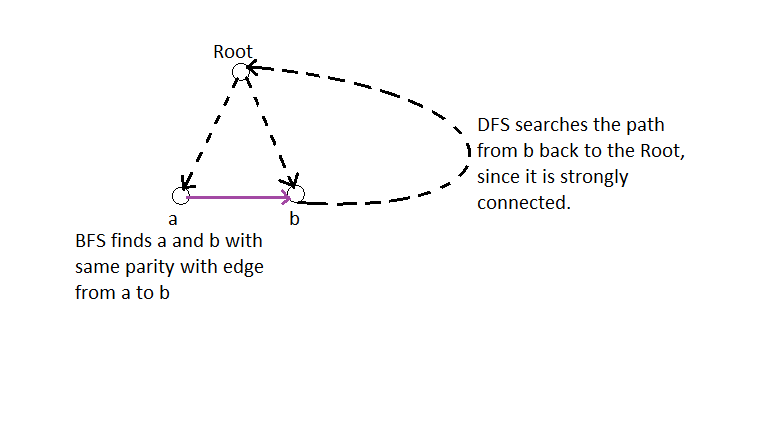
\includegraphics[width=8cm, height=8cm]{Prob4c}
  \caption{Finding the odd-cycle}
  \end{figure}

  Each node has a parity field. The root's parity field is marked as 0. For every node mark the parity of its children as its own parity's complement. Thus every node in the odd layer will have parity value of 1 and every node in the even layer will have a parity value of 0. If during the exploration using BFS we reach a node 'a', and discover an edge (a,b) where 'b' has already been discovered and marked with the same parity as that of 'a', that means , in the undirected version of the graph we have detected an odd cycle(bipartiteness test fails) namely Root $\rightarrow$ a $\rightarrow$ b $\rightarrow$ Root, but this excat cycle is not true for the directed case, since both a and b were reached from the Root along a forward moving path, and hence no cycle. However, we show that for a strongly connected directed graph, an odd cycle detection in its undirected version implies the existence of an odd cycle in its directed version and can be found by the mechanism described in this algorithm. Consider the following figure. \newline
  \begin{figure}[h!]
   \centering
  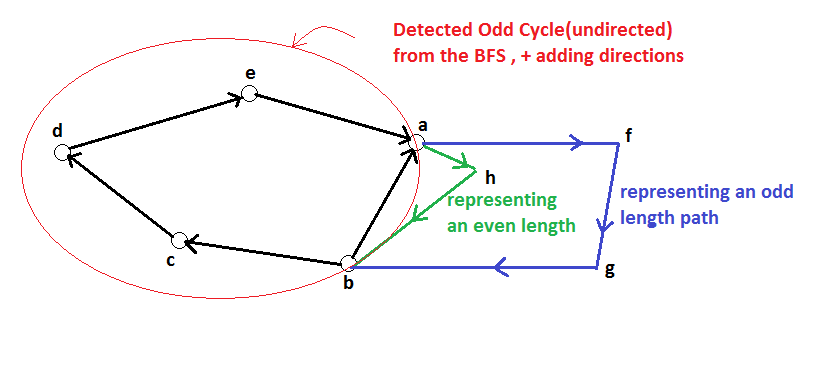
\includegraphics[width=15cm, height=8cm]{Prob4c_odd}
  \caption{Odd cycle of undirected graph with the reverese paths for strongly connected graph}
  \end{figure}

  a,b,c,d,e,a will result in an odd edge detection in the undirected graph. However, in the directed version, is a direction mismatch between e$\rightarrow$a and b$\rightarrow$a. But since it is a strongly connected graph, there will be another path from a$\rightarrow$b as well. The length of this path may be even, like a$\rightarrow$h$\rightarrow$b or odd, like a$\rightarrow$f$\rightarrow$g$\rightarrow$b. If the even size exists, then \textbf {a$\rightarrow$h$\rightarrow$b$\rightarrow$a} form an odd cycle. If the odd path exists, then \textbf {a$\rightarrow$f$\rightarrow$g$\rightarrow$b$\rightarrow$c$\rightarrow$d$\rightarrow$e$\rightarrow$a} is the odd cycle. \textbf {Thus there will always exist an odd cycle if the bipartiteness test fails.} We use this exact property to find the odd cycle. \newline
  Coming back to the point where we detected the existence of odd-cycle by parity matching(bipartiteness fails). We keep track of this edge (a,b), and terminate the BFS search here. Next, we start a DFS search to fiind the path from 'b' to the Root(Figure-2, this path exists since it is strongly connected and hence we are guaranteed to find this path using DFS). Once we find this path, the following cases are analyzed each of which is able to output an odd-cycle. \newline
  \hspace*{0.5cm} \textbf{If b$\rightarrow$Root is even length and Root$\rightarrow$b, which is of same parity as Root$\rightarrow$a, is odd length} : Then the odd cycle is \textbf {Root $\rightarrow$ b $\rightarrow$ Root} \newline
  \hspace*{0.5cm} \textbf{If b$\rightarrow$Root is even length and Root$\rightarrow$b, which is of same parity as Root$\rightarrow$a, is even length} : Then the odd cycle is \textbf {Root $\rightarrow$ a $\rightarrow$ b $\rightarrow$ Root} \newline
  \hspace*{0.5cm} \textbf{If b$\rightarrow$Root is odd length and Root$\rightarrow$b, which is of same parity as Root$\rightarrow$a, is odd length} : Then the odd cycle is \textbf {Root $\rightarrow$ a $\rightarrow$ b $\rightarrow$ Root} \newline
  \hspace*{0.5cm} \textbf{If b$\rightarrow$Root is odd length and Root$\rightarrow$b, which is of same parity as Root$\rightarrow$a, is even length} : Then the odd cycle is \textbf {Root $\rightarrow$ b $\rightarrow$ Root} \newline
The algorithm guarantees that if the odd-cycle is detected for the undirected graph it will find the correct odd-cycle for the strongly connected directed graph. It is trivial to note that if the undirected formation does not have an odd cycle, then the directed graph cannot have an odd-cycle as well.  \newline

\runtime 
   The main computation of the algorithm is centered around running the BFS followed by a DFS .  Both BFS and DFS takes $O(|E| + |V|)$ time. The rest of the computations are precisely about back tracking the search results produced by BFS and DFS to produce the final odd-cycles. These traversals will be $O(|E|)$. Additionally, the conditional blocks map to constant time operations. Thus, the overall running time of this algorithm is $O(|E| + |V|)$. \newline


\question{5}{Weary traveler \dots}
  Given there are n airports and m flights, the goal is to find the smallest total travel time from a source airport(S) to a destinations airport(d). \newline
We precisely apply the Dijkstra's algorithm to find the shortest path(in regards to travel time) with modifications in the mechanism to determine the cost of each path from one airport to another. The connectivity of the $m$ flights can be formed into a directed graph with edge(u,v) indicating the availability of a flight from u to v. Important to note here, is that from a port i there can be multiple direct flights to  another port 'j', and the m flights comprise of all such flights. Thus, unlike other problems where there is a single edge between two nodes in a specific direction and we treat the cardinality of the edges as the quantification of the connectivity of the nodes, in this case m does not directly implies the connectivity of the nodes. Each of these edges have an associated cost of flight duration. \newline
In addition to these, to determine the smallest travel time, one needs to consider the layover times at every airport. Also, we are given a constraint that there will always be a minimum layover of 10 mins. \newline
Consider a traveller arrives at airport 'i' at time 't', and we want to determine the flight it will take to go from 'i' to 'j' via the available direct flights, that is, in the directed graph, there are multiple edges from i to j and we need to decide which edge to consider for the travel. Suppose the available flights in the schedule from 'i' to 'j' , after the arrival time t, are as $[t_{ij,1}, t_{ij,2}, t_{ij,3}, \dots]$, and each of those flights have a flight duration of $[f_{ij,1}, f_{ij,2}, f_{ij,3}, \dots]$ where $t_{ij,k}$ indicates the start-time and $f_{ij,k}$ indicates the in-air flight duration of the k'th flight from 'i' to 'j'. We must choose that flight, which minimizes the combination of \textbf {layover + flight duration}. \newline
  Thus, we define the objective function, DURATION-COST, that can be written as: \newline
  \begin{equation}
	  DURATION-COST = min \bigg \{ \infty, \underset{k=1,2,..,h}{min}{\{t_{ij,k} - t + f_{ij,k}\}\bigg |_{t_{ij,k}-t \geq 10}}  \bigg \}
  \end{equation}

 This DURATION-COST is the modified cost of each path. Now we can apply Dijkstra's algorithm to find the shortest path of this graph using the cost function of equation(10), and that shortest path will correspond to the route for the smallest travel time. \newline

 \algo \newline
 \textbf {SmallestTimeTraveller(G, Source)}: \newline
 \hspace*{0.5cm} TimeCost[Source] = CurrentTime \newline
 \hspace*{0.5cm} \textbf {for} each $n \in Vertices$ \newline
 \hspace*{1.0cm} 	\textbf {if} (n is \textbf {not Source}) \newline
 \hspace*{1.5cm} 		TimeCost[n] = $\infty$ \newline
 \hspace*{1.5cm} 		Parent[n]   = Undef \newline
 \hspace*{1.0cm} 	\textbf {PriQueue}.add(n, TimeCost[n]) \newline
 \hspace*{0.5cm} \textbf {while} ( $\neg$ \textbf {PriQueue}.empty() ) \newline
 \hspace*{1.0cm} 	u = \textbf {PriQueue.extractMin()} // first only source will come, since others have cost infinity \newline
 \hspace*{1.0cm} 	\textbf {for} $v \in$ adjacencyList(u) \newline
 \hspace*{1.5cm} 		\textbf {DURATION-COST} = $ min \bigg \{ \infty, \underset{k=1,2,..,h}{min}{\{t_{ij,k} - TimeCost[u] + f_{ij,k}\}\bigg |_{t_{ij,k}-TimeCost[u] \geq 10}}  \bigg \}$ \newline
 \hspace*{1.5cm}		ExpectedTime = TimeCost[u] + DURATION-COST \newline
 \hspace*{1.5cm}		\textbf {if}(ExpectedTime $<$ TimeCost[v]) \newline
 \hspace*{2.0cm}			TimeCost[v] = ExpectedTime \newline
 \hspace*{2.0cm}			parent[v]   = u \newline
 \hspace*{2.0cm}			\textbf {PriQueue.update}(v, ExpectedTime) \newline
 \hspace*{0.5cm} \textbf {return} TimeCost, Parent \newline
 \newline

 \textbf {Analysis:}

 \runtime Here we use a heap based priority queue, for which each of the update and extractMin operation takes $O(\log n)$ time. In general, for  Dijkstra's algorithm run on a directed graph G of n nodes and m edges, is $O((m+n)\log n)$, however in these cases, each edge represents a valid path between two nodes that can be taken to travel in that route. In our case, there are suppossedly h possible direct paths between two nodes, out of which only one will be taken to evaluate the DURATION-COST, that is the one that minimizes the objective function. Thus, we have no way to find out the number of valid routes from m, however we can upper-bound that number by $n^2$, that is the worst case for a connected graph. \textbf {Additionally} we have the cost of minimizing the objective function at every node. Note that, at every node, we run a scan operation to find the minima of the objective function, which means at every node, all its outward degrees needs to be considered exactly once. Summing them up equals to all outgoing edges of the n nodes which is basically the total number of flights, 'm'. Thus the total running time is expressed as: \newline
\textbf {Running Time} = $O((n + n^2)\log n + m)$ = $O(n^2\log n + m)$ \newline

\correctness 
  Let R be the set of nodes for which the shortest travel time from Source,A, has been found. \textbf {Base-Case($|R|==1$):}  Since R only gets larger(no existence of negatove paths), the only time $|R|==1$ is when R={source} and TimeCost[source] = 0. Thus, base case is satisfied. \newline
  By inductive hypotheses, suppose for every vertex $v \in R$, we have found the shortest time of travel. Let u be the next node that is added to R, such that, $R^\prime = R \cup \{u\}$. TimeCost(v) denotes the shortest path in terms of time-travel cost from source to every $v \in R$. Suppose for contradiction, that the shortest path from source-to-u is Q and has cost length: \newline
  \[ l(Q) < TimeCost[u] \]
  This has two possibilites: \newline
  (1) Q starts in $R^\prime$, and leaves $R^\prime$ at some node and then reaches u. In this case, we assume that the minimizer of each route is correct and the only issue is in finding the shortest route. \newline
  (2) The flight path we had taken from the parent of the 'u', say k, to reach 'u' for the shortest path, was not optimal and there is a better flight option.  \newline
  We analyze below each of these cases separately: \newline
  \textbf {Case-1:} Let xy be the first edge along Q that leaves $R^\prime$. Let $Q_{x}$ be the route source$\rightarrow$x, which is a subpath of Q. Then the following holds:\newline
  \[ l(Q_{x} + l(x\rightarrow y) \leq l(Q) \]
  Since, x is in $R^\prime$, TimeCost[x] is the travel time of the shortest path source-to-x , and by the induction hypotheses, \newline
  \[ TimeCost[x] \leq l(Q_{x}) \]
  Then, replacing in the previous equation, we get, \newline
  \[ TimeCost[x] + l(x\rightarrow y) \leq l(Q) \]
  Since, y is adjacent to x, TimeCost[y] must have been updates by the algorithm as : \newline
  \[ TimeCost[y] \leq TimeCost[x] + l(x \rightarrow y) \]
  Finally, since 'u' was picked by the algorithm, and y was not chosen until the current step, this implies: \newline
  \[ TimeCost[u] < TimeCost[y] \]
  Back substituting this expressions in the previous ones, we get: \newline
  \[ TimeCost[u] < TimeCost[u] \]
  which is a clear contradiction. Thus, TimeCost[u] is the shortest travel time from source-to-u, given our minimization function across multiple flights between two nodes is correct(we address this issue in the next case).  \newline
  \textbf {Case-2:} Let us consider again a contradiction that there exists a flight path from the parent(k) of 'u' to 'u' that would have given a better minimal time for 'u'. Since our objective function,'DURATION-COST', is a minimizer over all the possible flights from 'k' to 'u' for flights that start after TimeCost[k]+10, then the only possibility of getting a shorter flight in this route is of the traveller arrives at 'k' before TimeCost[k]. However, by our inductive hypotheses, all the nodes in R are already at their minimal travel time cost, hence it is \textbf {not possible} to arrive at 'k' earlier than TimeCost[k]. Hence, the chosen flight from 'k' to 'u' is the optimal flight that minimizes the travel time cost for source-to-u. \newline
  The above two cases guarantees the correctness of the algorithm. \newline

\end{document} 
